\documentclass[12pt]{article} %set font size and document type
\usepackage{graphicx} % Required for inserting images
\usepackage[useregional]{datetime2} %allow use of \today
\usepackage[margin=1in]{geometry} % set margins
\usepackage{setspace} % allow setting of double and single spacing
\usepackage{hyperref} % creates clickable table of contents
\usepackage{adjustbox} % allows us to rotate images, tables, etc.
\usepackage{float}

% \usepackage{xcolor}
\usepackage{color, colortbl}

\usepackage{listings}
\newcommand{\lsin}[1]{\lstinline[columns=fullflexible,keepspaces=true,language=Java,basicstyle=\footnotesize\ttfamily]{#1}}

\lstdefinelanguage{Java}{
  columns=fullflexible,keepspaces=true,basicstyle=\scriptsize\ttfamily,
%  basicstyle=\scriptsize\sffamily,
  numbers=left,
  xleftmargin=5.0ex,
  escapechar=@,
  sensitive=true,
  otherkeywords={},
  morekeywords=[1]{int,while,if,public,static,else,return,new,for,return,void},
  keywordstyle={[1]\bfseries\color{blue}},
  numberstyle=\tiny\color{black},
  rulecolor=\color{black},
}

% set up header and footer
\usepackage{titleps,kantlipsum}
\newpagestyle{mypage}{%
  \headrule
  \sethead{\MakeUppercase{\thesection\quad \sectiontitle}}{}{\thesubsection\quad \subsectiontitle}
  \setfoot{}{}{\em{p. \thepage}}
}
\settitlemarks{section,subsection}
\pagestyle{mypage}

% set up title information 
% Students replace project title and their names here
\title{Crazy Eights
\\
CS482 Software Engineering}
\author{William Grimmer, Jack Formato, Victoria Shelton\\
Client: Eric Ebert}
\date{\today}

\begin{document}

\maketitle

% creates table of contents
\pagebreak
\tableofcontents
\section*{Abstract}



%[[ text between `[[' and `]]' are comments from me to you and should be commented out as you complete various section 

%Put here the \emph{elevator pitch} for your project. 

%IOW a 1-2 paragraph summary of your project that includes who the client is and why they need this App.]]

The Crazy Eights project is a web app that allows users to play the Crazy Eights card game. Users can create accounts and log in to keep track of their games and statistics. They can also send friend requests to users, which once accepted by the recipient, allows them to message that user. Users can choose to host or join a multiplayer game of Crazy Eights, and are given options to choose a public or private game, as well as the buy-in they are willing to spend. Once a game is started, each user can act on their turn until the game won or lost.

This project was requested by the client, Eric Ebert, on behalf of `XYZ Enterprises.' He wanted this website created for the purposes of monetizing the game and bringing in more money to his company. The main way the website generates income is through non-intrusive ads.



\pagebreak
% make body of document double spaced for easier feedback writing
% \doublespacing 


% include the latex files with the content
\section{Introduction}

%[[ No more than one page that provides a short project description and then sets the stage for the rest of the document. ]]

%This sentence has an example citation~\cite{DBLP:journals/infsof/BinkleyMI22}


%Introduce your project to your reader by describing your client’s needs, providing a high-level overview of your software solution, and presenting an outline of the rest of your document. Your Introduction should be about a single spaced page

This project is a website that allows users to play the Crazy Eights card game with other users. It was completed for the client Eric Ebert. The client requested that the website have account functionality such as creating accounts, signing in, befriending other users, and messaging other users. The website should also have admins that can assist users with resetting their passwords and changing other account information. Users should be able to create reports to request assistance from admins if they encounter a user who is misbehaving. Users can play as a guest, but an account is needed if they wish to collect virtual currency and review their statistics.

To play a game, users should be able to host a game or join a game. Hosts should be able to specify the settings for their games, as well as choosing if their game should be public or private through setting a password. Those who wish to join a game must provide the correct password to be allowed access. The client also specified that the website should contain the company's name. The website should also have ads for monetary purposes, but not to the point where it would drive a potential user away. The client also requested that the game should have a virtual currency and a betting component.

Our solution to the client's requests was to build a website using three-tiered architecture. The server would be built using Nodejs, the client would be created with React, and the database would be hosted on Firebase. Our original plan was to use SQL to host the database, but Firebase became the easier alternative because it had free hosting options. In addition, we used existing frameworks and libraries like Expressjs for backend setup, Socketio for multiplayer functionality, and Bootstrap for template UI elements. This stack allowed us to build our website efficiently, and assign each of the three layers to one person.

We implemented the client's requests with several different webpages. The main page allowed users to host a game, join a game, and access account options. The account pages allowed users to create an account, log in to an account, and view their account. On the view account page, users could view their statistics, send/accept friend requests, send/read messages, and create reports. The create game page allowed users to specify the settings for their game, and start the game once enough players joined the lobby. The join game page showed users the list of currently active lobbies that they could join, as well as if they required a password to join. Lastly, the game page held the functionality for the Crazy Eights card game, allowing users to play against others and win or lose.

Some of the clients requests were not able to be implemented due to compatibility or time constraints. For example, the client requested that betting with virtual currency should be an option. However, Crazy Eights is not a gambling game, and is not formatted for gambling. So, we decided that each game would have a buy-in determined by the host. Additionally, the client requested that hosts should determine the amount of bots when creating a game. We were not able to implement bots with the amount of time we had.

This document will provide an overview of our process and work during the semester. It will include the user stories and requirements specified by the client, data on each of the three sprints, the architecture and design decisions, testing process, database persistence, and a reflection on the project.
\section{Requirements}

\subsection{User Roles}


\subsubsection{Player}
A player is a user who has created an account and has access to view their own profile. A player can create games, join games, change their own password, add friends, message their friends and report other players. This user has no technical expertise and has standard level access.

\subsubsection{Admin}
An admin is a user who has an account created for them, granting them special permissions on sign in. In addition to having the same functionality as a player, the admin can, view reports, resolve reports and delete player accounts. An admin needs to be familiar with the technical no how of dealing with reports and has a high level of access.



\subsection{Functional Requirement User Stories and Tasks}

We chose to organize our user stories by user type and Story ID. Story ID's were organized alphabetically to easily find related user stories as well as improve readability.


\subsubsection{Player}

\textbf{A0: Log in to account (2)}
\begin{enumerate}
    \item Priority: High
    \item \textbf{I want} to log into my account
    \item \textbf{So that} I can use my account
    \item \textbf{Definition of Done:} When the player can access their account
    \item \textbf{Depends On:} A1: Make an account
    \item Tasks:
    \begin{enumerate}
    % For each task write the ID, :, then title. Then describe the task.
        \item Task [[ A0.1: login form. Create login form page.]]
        \item Task [[ A0.2: connect to database. authenticate credentials against backend credentials.]]
        \item Task [[ A0.3: Session management. create persistence for session that continues as user navigates the website.]]
    \end{enumerate}
\end{enumerate}

\vspace{2em}

\textbf{A1: Make an account (2)}
\begin{enumerate}
    \item Priority: High
    \item \textbf{I want} to make an account
    \item \textbf{So that} I can keep track of my stats
    \item \textbf{Definition of Done:} when the account is added to the database
    \item \textbf{Depends On:} Nothing
    \item Tasks:
    \begin{enumerate}
    % For each task write the ID, :, then title. Then describe the task.
        \item Task [[ A1.1: Create registration form. Create page to make an account.]]
        \item Task [[ A1.2: Propogate account in database. make sure account generates in the DB.]]
    \end{enumerate}
\end{enumerate}

\vspace{2em}

\textbf{A2: Update my account (2)}
\begin{enumerate}
    \item Priority: Medium
    \item \textbf{I want} to update my account
    \item \textbf{So that} I can change my information
    \item \textbf{Definition of Done:} the database gets the update
    \item \textbf{Depends On:} A1: Make an account
    \item Tasks:
    \begin{enumerate}
    % For each task write the ID, :, then title. Then describe the task.
        \item Task [[ A2.1: create update page. create form to update the users data.]]
        \item Task [[ A2.2: Modify database correctly. make sure the correct user is changed and data is updated in real time.]]
    \end{enumerate}
\end{enumerate}

\vspace{2em}

\textbf{A3: Delete account (2)}
\begin{enumerate}
    \item Priority: Low
    \item \textbf{I want} to delete my account
    \item \textbf{So that} I can remove an account
    \item \textbf{Definition of Done:} When the account is removed from the database
    \item \textbf{Depends On:} A1: Make an account
    \item Tasks:
    \begin{enumerate}
    % For each task write the ID, :, then title. Then describe the task.
        \item Task [[ A3.1: Admin panel to delete account. create the panel from which accounts can be deleted.]]
        \item Task [[ A3.2: Remove from database. ensure that user has been removed from database .]]
    \end{enumerate}
\end{enumerate}

\vspace{2em}

\textbf{A4: Check account information (2)}
\begin{enumerate}
    \item Priority: High
    \item \textbf{I want} to view account info/balance
    \item \textbf{So that} I know my balance
    \item \textbf{Definition of Done:} The player can see their account information
    \item \textbf{Depends On:} A1: Make an account
    \item Tasks:
    \begin{enumerate}
    % For each task write the ID, :, then title. Then describe the task.
        \item Task [[ A4.1: create users page. Allow users to view their own profile]]
        \item Task [[ A0.1: Load session information. load correct information from user logged in, update from DB as it changes.]]
    \end{enumerate}
\end{enumerate}

\vspace{2em}

\textbf{H0.1: Create Lobby (5)}
\begin{enumerate}
    \item Priority: High
    \item \textbf{I want} to make a lobby
    \item \textbf{So that} other people can join
    \item \textbf{Definition of Done:} When the lobby is created and available to join
    \item \textbf{Depends On:} Nothing
    \item Tasks:
    \begin{enumerate}
    % For each task write the ID, :, then title. Then describe the task.
        \item Task [[ H0.1.1: Create Lobby Form. Build a form to configure and create a lobby.]]
        \item Task [[ H0.1.2: Connect players. make sure players are connected to lobby so they can interact with each other.]]
    \end{enumerate}
\end{enumerate}

\vspace{2em}

\textbf{H0.2: Start Game (5)}
\begin{enumerate}
    \item Priority: High
    \item \textbf{I want} to start the game
    \item \textbf{So that} we can play the game
    \item \textbf{Definition of Done:} The game starts
    \item \textbf{Depends On:} H0.1: Create Lobby
    \item Tasks:
    \begin{enumerate}
    % For each task write the ID, :, then title. Then describe the task.
        \item Task [[ H0.2.1: Create start game button. Button available to host of game to start]]
    \end{enumerate}
\end{enumerate}

\vspace{2em}

\textbf{H0.3: Leave Game (1)}
\begin{enumerate}
    \item Priority: Medium
    \item \textbf{I want} to leave the game
    \item \textbf{So that} I can get back to the home page
    \item \textbf{Definition of Done:} When I can go back to the home page and leave the game room
    \item \textbf{Depends On:} H0.1: Create Lobby, H0.2: Start Game, P7: Join Game
    \item Tasks:
    \begin{enumerate}
    % For each task write the ID, :, then title. Then describe the task.
        \item Task [[ H0.3.1: Create button to leave game. Button to leave game]]
        \item Task [[ H0.3.2: Remove user from the lobby. Kick the user from the game and return them to the home screen.]]
    \end{enumerate}
\end{enumerate}

\vspace{2em}

\textbf{P1: Play a card (5)}
\begin{enumerate}
    \item Priority: High
    \item \textbf{I want} to place a card
    \item \textbf{So that} the game can progress
    \item \textbf{Definition of Done:} When a card leaves my hand
    \item \textbf{Depends On:} H0.2: Start Game
    \item Tasks:
    \begin{enumerate}
    % For each task write the ID, :, then title. Then describe the task.
        \item Task [[ P1.1: Allow user to select card. Select card so it can be placed o top of deck]]
        \item Task [[ P1.2: Check if card can be placed on deck. Logic to define if card place is valid]]
    \end{enumerate}
\end{enumerate}

\vspace{2em}

\textbf{P1.1: End Game (2)}
\begin{enumerate}
    \item Priority: High
    \item \textbf{I want} to end the game
    \item \textbf{So that} I can get a win/loss
    \item \textbf{Definition of Done:} When the game ends and player stats are updated
    \item \textbf{Depends On:} H0.2: Start Game, P1: Play Card
    \item Tasks:
    \begin{enumerate}
    % For each task write the ID, :, then title. Then describe the task.
        \item Task [[ P1.2: If user has no cards end game. Checks if cards are empty and ends game if so]]
    \end{enumerate}
\end{enumerate}

\vspace{2em}

\textbf{P2: Draw a card (5)}
\begin{enumerate}
    \item Priority: High
    \item \textbf{I want} to draw a card
    \item \textbf{So that} the game can progress
    \item \textbf{Definition of Done:} I get a new card in my hand
    \item \textbf{Depends On:} H0.2: Start Game
    \item Tasks:
    \begin{enumerate}
    % For each task write the ID, :, then title. Then describe the task.
        \item Task [[ P2.1: User click on deck. Click on deck so they can draw card]]
        \item Task [[ P2.2: If deck is clicked, update users hand. adds card to users hand if deck is clicked]]
    \end{enumerate}
\end{enumerate}

\vspace{2em}

\textbf{P5: Tutorial (1)}
\begin{enumerate}
    \item Priority: Low
    \item \textbf{I want} to learn the game
    \item \textbf{So that} I can understand the game
    \item \textbf{Definition of Done:} I am sent to the rules page
    \item \textbf{Depends On:} Nothing
    \item Tasks:
    \begin{enumerate}
    % For each task write the ID, :, then title. Then describe the task.
        \item Task [[ P5.1: Create button to link of rules. Button is hyperlinked to external site that includes rules of the game ]]
    \end{enumerate}
\end{enumerate}

\vspace{2em}

\textbf{P6: View Games (5)}
\begin{enumerate}
    \item Priority: High
    \item \textbf{I want} to view all joinable games
    \item \textbf{So that} I can join a game
    \item \textbf{Definition of Done:} I can see all the joinable games
    \item \textbf{Depends On:} H0.1: Create Lobby
    \item Tasks:
    \begin{enumerate}
    % For each task write the ID, :, then title. Then describe the task.
        \item Task [[ P6.1: Create games page. Create page to show games ]]
        \item Task [[ H6.2: Load games. Load list of all available games]]
    \end{enumerate}
\end{enumerate}

\vspace{2em}

\textbf{P7: Join Game (8)}
\begin{enumerate}
    \item Priority: High
    \item \textbf{I want} to join a game
    \item \textbf{So that} to play with other users
    \item \textbf{Definition of Done:} When I join a lobby
    \item \textbf{Depends On:} H0.1: Create Lobby
    \item Tasks:
    \begin{enumerate}
    % For each task write the ID, :, then title. Then describe the task.
        \item Task [[ P7.1: Create join game button. Button that joins game]]
        \item Task [[ P7.2: Check password. check to make sure game password is correct]]
    \end{enumerate}
\end{enumerate}

\vspace{2em}

\textbf{P7.1: Connect Users to Game (2)}
\begin{enumerate}
    \item Priority: Low
    \item \textbf{I want} to join a game through my account
    \item \textbf{So that} I can keep track of my stats
    \item \textbf{Definition of Done:} When users are tracked by games
    \item \textbf{Depends On:} A1: Make an account, A0: Log in to account, H0.1: Create Lobby
    \item Tasks:
    \begin{enumerate}
    % For each task write the ID, :, then title. Then describe the task.
        \item Task [[ P7.1.1: Connect to game. If password is correct, connect to lobby]]
    \end{enumerate}
\end{enumerate}

\vspace{2em}

\textbf{P9: Ads (3)}
\begin{enumerate}
    \item Priority: Low
    \item \textbf{I want} to click on an ad
    \item \textbf{So that} I can go to the link
    \item \textbf{Definition of Done:} When I can go to the link for an ad by clicking it
    \item \textbf{Depends On:} Nothing
    \item Tasks:
    \begin{enumerate}
    % For each task write the ID, :, then title. Then describe the task.
        \item Task [[ P9.1: Show ads on home page. display ads with hyperlink on homepage]]
    \end{enumerate}
\end{enumerate}

\vspace{2em}

\textbf{P10: Send Message (5)}
\begin{enumerate}
    \item Priority: Medium
    \item \textbf{I want} to send a message
    \item \textbf{So that} I can communicate with others
    \item \textbf{Definition of Done:} When user can DM other players
    \item \textbf{Depends On:} P13: Add friend
    \item Tasks:
    \begin{enumerate}
    % For each task write the ID, :, then title. Then describe the task.
        \item Task [[ P10.1: View message modal. Display the message modal between friends]]
        \item Task [[ P10.2: Send content to DB. Send content entered in form to the database]]
    \end{enumerate}
\end{enumerate}

\vspace{2em}

\textbf{P11: Read Message (5)}
\begin{enumerate}
    \item Priority: Medium
    \item \textbf{I want} to read my messages
    \item \textbf{So that} I can see what other players have DMed ne
    \item \textbf{Definition of Done:} When user can view all messages sent to them
    \item \textbf{Depends On:} A1: Make an account, P10: Send Message, P13: Add friend
    \item Tasks:
    \begin{enumerate}
    % For each task write the ID, :, then title. Then describe the task.
        \item Task [[ P11.1: View message modal. Display the message modal between friends]]
        \item Task [[ P11.2: Load messages. Pull existing messages from the database]]
    \end{enumerate}
\end{enumerate}

\vspace{2em}

\textbf{P12: Report (3)}
\begin{enumerate}
    \item Priority: Low
    \item \textbf{I want} to report another player
    \item \textbf{So that} bad accounts are seen by admins
    \item \textbf{Definition of Done:} When the report is sent
    \item \textbf{Depends On:} A1: Make an account
    \item Tasks:
    \begin{enumerate}
    % For each task write the ID, :, then title. Then describe the task.
        \item Task [[ P12.1: Create report button. Button that opens form to report]]
        \item Task [[ P12.2: Send report form. Send form to database containing user and issue]]
    \end{enumerate}
\end{enumerate}

\vspace{2em}

\textbf{P13: Add friend (3)}
\begin{enumerate}
    \item Priority: Low
    \item \textbf{I want} to add a friend
    \item \textbf{So that} I can ask someone to be a friend
    \item \textbf{Definition of Done:} When a friend request is sent
    \item \textbf{Depends On:} A0: Log in to account, A1: Make an account
    \item Tasks:
    \begin{enumerate}
    % For each task write the ID, :, then title. Then describe the task.
        \item Task [[ P13.1: Create add friend button. Button that adds friend by username]]
        \item Task [[ P13.2: Logic to find friend in DB. Search database for username given]]
        \item Task [[ P13.3: Make friend request if friend found. If the username exists, create a friend request in that users friend request array in the database]]
    \end{enumerate}
\end{enumerate}

\vspace{2em}

\textbf{P14: Accept friend (1)}
\begin{enumerate}
    \item Priority: Low
    \item \textbf{I want} to accept a friend request
    \item \textbf{So that} I can have a friend
    \item \textbf{Definition of Done:} Friends are saved in database and displayed on page
    \item \textbf{Depends On:} P13: Add friend
    \item Tasks:
    \begin{enumerate}
    % For each task write the ID, :, then title. Then describe the task.
        \item Task [[ P14.1: Load friend requests. Form that shows and loads users friend requests]]
        \item Task [[ P14.2: Accept friend. button to accept and create friend relationship]]
        \item Task [[ P14.3: Remove friend request. Delete the friend request from DB now that it has been accepted]]
    \end{enumerate}
\end{enumerate}

\subsubsection{Admin}

\textbf{M2: Read player report (1)}
\begin{enumerate}
    \item Priority: Low
    \item \textbf{I want} to read a report
    \item \textbf{So that} I can check if a player is misbehaving
    \item \textbf{Definition of Done:} Report is read
    \item \textbf{Depends On:} P12: Report
    \item Tasks:
    \begin{enumerate}
    % For each task write the ID, :, then title. Then describe the task.
        \item Task [[ M2.1: View reports. Load active reports into form]]
        \item Task [[ M2.2: Resolve report. Button that removes report from database once resolved]]
    \end{enumerate}
\end{enumerate}

\vspace{2em}

\textbf{M4: Change password (3)}
\begin{enumerate}
    \item Priority: Low
    \item \textbf{I want} to change my password
    \item \textbf{So that} my account stays safe
    \item \textbf{Definition of Done:} When password is changed in the database
    \item \textbf{Depends On:} A1: Make an account
    \item Tasks:
    \begin{enumerate}
    % For each task write the ID, :, then title. Then describe the task.
        \item Task [[ M4.1: View users button. Shows all active users and their ids]]
        \item Task [[ M4.2: Button to change password on each user. Button that opens form to change password of said user]]
        \item Task [[ M4.3: Save changes. Saves changed password to the DB]]
    \end{enumerate}
\end{enumerate}
\subsection{Non-Functional Requirements}

\subsubsection{Category: User Interface}

\textbf{ID: UI Improvement for Game Interface}
\begin{enumerate}
\item Description: Enhance the game interface to make the cards and win/lose screen more appealing.
\item Affects: End users interacting with the game
\end{enumerate}


\textbf{ID: UI Improvement for Admin Panel}
\begin{enumerate}
\item Description: Upgrade the admin panel's design and layout to make differentiating between users easier
\item Affects: Administrators managing the system
\end{enumerate}


\subsubsection{Category: Security}

\textbf{ID: Ensuring Valid Email}
\begin{enumerate}
\item Description: Ensures users cannot register for an account without a valid email
\item Affects: User registration process
\end{enumerate}


\subsubsection{Category: Performance}

\textbf{ID: Switching Database to NoSQL for Speedup}
\begin{enumerate}
\item Description: Migrate the database to a NoSQL version on firebase for faster access and easier hosting
\item Affects: Backend database operations and system performance.
\end{enumerate}


\section{Iterations}

[[ The requirements analysis identifies \textbf{what} your client wants.
With each iteration describe the \textbf{how}.
Include user stories attempted, data structures introduced, and any key design
decisions.

Copy this layout for each iteration. ]]

\subsection{Overview}

To complete this project, we split the stories into three two-week sprints. Table \ref{Table 1} illustrates the spread of story points in each sprint. This includes total points, remaining points at the start of the sprint, the points attempted in that sprint, and the points completed in that sprint. If a story was not complete, the points were not included in the completed column and are attempted in a later sprint. In addition, the total points increased in Sprint 3 because we added slices to previous user stories. The table also includes the team's speed (story points per sprint) and cycle time (hours-per-point per story point). The averages for these are included in the final row with averages for attempted points and completed points.

\begin{table}[h]
\resizebox{\textwidth}{!}{%
\begin{tabular}{|c|c|c|c|c|c|c|}
\hline
\textbf{Sprint} & \textbf{Total Points} & \textbf{Remaining Points} & \textbf{Attempted Points} & \textbf{Completed Points} & \textbf{Speed} & \textbf{Cycle Time} \\ \hline
1               & 69                    & 69                        & 28                        & 18                        & 18             & 2.71                \\ \hline
2               & 69                    & 51                        & 38                        & 30                        & 24             & 2.05                \\ \hline
3               & 73                    & 25                        & 25                        & 25                        & 24.33          & 2.6                 \\ \hline
Average         & -                     & -                         & 30.33                     & 24.33                     & 22.11          & 2.45                \\ \hline
\end{tabular}
}
\caption{Project overview}
\label{Table 1}
\end{table}



\subsection{Iteration 1}

\subsubsection{Plan}
The team's plan for Sprint 1 was to get a basic framework for the important aspects of the project. We started by slicing a story, "Create Game". This story was too large, and we had overestimated its story points. To solve this, we split it into three stories: "Create Lobby", "Start Game", and "Leave Game". Originally "Create Game" was 13 points. This was changed to a total of 11 points between the three slices. This change made the task ahead clearer and emphasized that the lobby and game pages were separate. Table \ref{Table 2} breaks down each story attempted in Sprint 1. Each team member took stories related to the layer that they were going to focus on. Victoria worked with the UI, Jack focused on the backend, and Will connected the database. The plan was for each to learn one layer the best so that he or she could help the others when needed.

\begin{table}[h]
\centering
\begin{tabular}{|c|c|c|c|c|}
\hline
\textbf{ID} & \textbf{Story}            & \textbf{Team Member} & \textbf{Points} & \textbf{Status} \\ \hline
H0.1 & Create Lobby              & Victoria    & 5      & Not Accepted \\ \hline
H0.2 & Start Game                & Victoria    & 5      & Accepted     \\ \hline
P1   & Play a card               & Jack        & 5      & Not Accepted \\ \hline
P2   & Draw a card               & Jack        & 5      & Accepted     \\ \hline
A1   & Make an account           & Will        & 2      & Accepted     \\ \hline
A4   & Check account information & Will        & 2      & Accepted     \\ \hline
A2   & Update my account         & Will        & 2      & Accepted     \\ \hline
A3   & Delete account            & Will        & 2      & Accepted     \\ \hline
\end{tabular}
\caption{Sprint 1 stories}
\label{Table 2}
\end{table}


\begin{table}[h]
\begin{tabular}{|ccccc|}
\hline
\multicolumn{5}{|c|}{\textbf{Sprint 1}}                                                                                                                                                                  \\ \hline
\multicolumn{1}{|c|}{\textbf{Team Member}} & \multicolumn{1}{c|}{\textbf{Attempted Points}} & \multicolumn{1}{c|}{\textbf{Completed Points}} & \multicolumn{1}{c|}{\textbf{Speed}} & \textbf{Cycle Time} \\ \hline
\multicolumn{1}{|c|}{Victoria}             & \multicolumn{1}{c|}{10}                        & \multicolumn{1}{c|}{5}                         & \multicolumn{1}{c|}{5}              & 3                   \\ \hline
\multicolumn{1}{|c|}{Jack}                 & \multicolumn{1}{c|}{10}                        & \multicolumn{1}{c|}{5}                         & \multicolumn{1}{c|}{5}              & 3                   \\ \hline
\multicolumn{1}{|c|}{Will}                 & \multicolumn{1}{c|}{8}                         & \multicolumn{1}{c|}{8}                         & \multicolumn{1}{c|}{8}              & 2                   \\ \hline
\multicolumn{5}{|c|}{\textbf{Total}}                                                                                                                                                                     \\ \hline
\multicolumn{1}{|c|}{Victoria}             & \multicolumn{1}{c|}{10}                        & \multicolumn{1}{c|}{5}                         & \multicolumn{1}{c|}{5}              & 3                   \\ \hline
\multicolumn{1}{|c|}{Jack}                 & \multicolumn{1}{c|}{10}                        & \multicolumn{1}{c|}{5}                         & \multicolumn{1}{c|}{5}              & 3                   \\ \hline
\multicolumn{1}{|c|}{Will}                 & \multicolumn{1}{c|}{8}                         & \multicolumn{1}{c|}{8}                         & \multicolumn{1}{c|}{8}              & 2                   \\ \hline
\end{tabular}
\caption{Team member points for Sprint 1}
\label{Table 3}
\end{table}


\subsubsection{Activities}
Victoria started by making React pages and linking them through buttons on the home page. She made pages for the home page, lobby, game, and account. Victoria's user stories are shown in Table \ref{Table 2}. The lobby page contained different fields for setting the name of the room, a bet, whether it was public or private, and a password. The game page was filled with the back of a card for the deck, a face-up card for the pile, and a line of cards as the player's hand. She also worked with Jack to make the game in the backend as well. 

Jack's stories had to do with the player actions. He wrote the classes for Player, Game, Deck, and Card. To connect to the frontend he used SocketIO. This gave the frontend the ability to call functions backend functions, as well as allowing the backend to give the frontend alerts as needed. SocketIO would also keep track of the user's session through different pages, so that we could keep their information consistent. Jack's user stories are shown in Table \ref{Table 2}. Both "Play a card" and "Draw a card" used the socket connection to function.

Will worked on the database. He used MySQL in his implementation. Using express he made post calls to the database to fetch and update information from the database. His stories in Table \ref{Table 2}, were the CRUD for the database. With Victoria, Will helped to write the code for the account. He was able to make, display, update, and delete accounts on this page.

\subsubsection{Retrospective}
Sprint 1 was a good learning experience. We should’ve started earlier, but struggled too because of other work. The biggest issue we had was that underestimated the time it would take for the initial setup. We also had to learn JavaScript and React syntax for the first time. Table \ref{Table 3} illustrates the progress made in this sprint. Two stories were not accepted. These were "Create Lobby" and "Play a card". We completed most of these two stories, but small parts weren't complete. The lobby page needed to be improved and take in the user's input and playing an eight didn't allow the user to pick the suit. These had to be finished in a later sprint. We also realized that there are no free SQL databases. We decided that it would be better to move to Firebase and use NoSQL for this reason.


\subsection{Iteration 2}

\subsubsection{Plan}
The plan for Sprint 2 was to finish important functionality. We took on the stories that were not accepted in Sprint 1, and worked toward multiplayer. Table \ref{Table 4} contains these stories. We worked to connect players through messages, friends, and multiplayer games. This sprint, we planned to take a large chunk of the stories because we knew that we would be able to complete more with the setup done. Team members took similar stories to Sprint 1. Will will continue to work with the database. He planned to switch to Firebase and worked toward being able to log in and change a user's password. Jack took stories to continue developing the game. His goal was to add multiple players to the same game. Victoria will continue the UI with "View Games", but also interact with the database when making friends.

\begin{table}[h]
\centering
\begin{tabular}{|c|c|c|c|c|}
\hline
\textbf{ID} & \textbf{Story}    & \textbf{Team Member} & \textbf{Points} & \textbf{Status} \\ \hline
H0.1 & Create Lobby      & Victoria    & 5      & Accepted     \\ \hline
P6   & View Games        & Victoria    & 5      & Accepted     \\ \hline
P13  & Add friend        & Victoria    & 3      & Not Accepted \\ \hline
P14  & Accept friend     & Victoria    & 1      & Accepted     \\ \hline
P1   & Play a card       & Jack        & 5      & Accepted     \\ \hline
P7   & Join Game         & Jack        & 8      & Accepted     \\ \hline
H0.3 & Leave game        & Jack        & 1      & Accepted     \\ \hline
A0   & Log in to account & Will        & 2      & Accepted     \\ \hline
M4   & Change password   & Will        & 3      & Not Accepted \\ \hline
P11  & Read message      & Will        & 5      & Not Accepted \\ \hline
\end{tabular}
\caption{Sprint 2 stories}
\label{Table 4}
\end{table}

\begin{table}[h]
\begin{tabular}{|ccccc|}
\hline
\multicolumn{5}{|c|}{\textbf{Sprint 2}}                                                                                                                                                                  \\ \hline
\multicolumn{1}{|c|}{\textbf{Team Member}} & \multicolumn{1}{c|}{\textbf{Attempted Points}} & \multicolumn{1}{c|}{\textbf{Completed Points}} & \multicolumn{1}{c|}{\textbf{Speed}} & \textbf{Cycle Time} \\ \hline
\multicolumn{1}{|c|}{Victoria}             & \multicolumn{1}{c|}{14}                        & \multicolumn{1}{c|}{11}                        & \multicolumn{1}{c|}{11}             & 2.5                 \\ \hline
\multicolumn{1}{|c|}{Jack}                 & \multicolumn{1}{c|}{14}                        & \multicolumn{1}{c|}{14}                        & \multicolumn{1}{c|}{14}             & 2                   \\ \hline
\multicolumn{1}{|c|}{Will}                 & \multicolumn{1}{c|}{10}                        & \multicolumn{1}{c|}{2}                         & \multicolumn{1}{c|}{2}              & 1.5                 \\ \hline
\multicolumn{5}{|c|}{\textbf{Total}}                                                                                                                                                                     \\ \hline
\multicolumn{1}{|c|}{Victoria}             & \multicolumn{1}{c|}{19}                        & \multicolumn{1}{c|}{16}                        & \multicolumn{1}{c|}{8}              & 3.42                \\ \hline
\multicolumn{1}{|c|}{Jack}                 & \multicolumn{1}{c|}{19}                        & \multicolumn{1}{c|}{19}                        & \multicolumn{1}{c|}{9.5}            & 3.05                \\ \hline
\multicolumn{1}{|c|}{Will}                 & \multicolumn{1}{c|}{18}                        & \multicolumn{1}{c|}{10}                        & \multicolumn{1}{c|}{5}              & 2                   \\ \hline
\end{tabular}
\caption{Team member points for Sprint 2}
\label{Table 5}
\end{table}

\subsubsection{Activities}
Victoria finished "Create Lobby" this sprint. She passed the game's name, bet, public status, and password through the socket. Table \ref{Table 4} illustrates the stories that Victoria worked on. Other than "Create Lobby", she worked to make a new React page for viewing games. This connected directly with Jack's user stories making it an important addition. She also worked towards adding friends which created connections in the database.

Jack decided to refactor the classes. First, he moved them into their own files and then cut out any unnecessary functions and variables. This was done to be more readable and efficient. His user stories from Table \ref{Table 4} were to join and leave games. This was done through socket rooms. When a game was made, a new room would be created using the game's name. All players would join this room to receive updates during the game. SocketIO allows for alerts to be sent to all socket connections within a specific room. This was used to tell the frontend when someone had played a card.

Will switched the database to Firebase. Firebase was free and allowed everyone to fetch from it, unlike MySQL. He then added new calls to the database to log in and change a password. The plan was for Will to work on send and read messages, but changing databases took too long. This led to "Send Message" not being attempted, and "Read Message" not being accepted. This is shown in Table \ref{Table 4}.

\subsubsection{Retrospective}
This sprint was successful, but left the team with a few issues. The first being that
most of the user stories were done very literally. An example of this is "Play a card", which is completed, but didn’t cover ending the game when someone won. In the next sprint we will make some slices to fix these gaps, and make sure the game runs smoothly. Testing was another issue we faced. We found it difficult to mock React and SocketIO in Jest. This hindered our branch coverage. We wish we figured it out sooner. Next sprint, we will put more emphasis on testing and make tests much earlier in the sprint. We realized that Will took on too much this sprint which stopped him from completing all of his stories. We should have made a technical task for converting the database to Firebase. This affected his speed in Table \ref{Table 5}.


\subsection{Iteration 3}

\subsubsection{Plan}
For Sprint 3 we made several slices of user stories and a technical task. Firstly, we made a slice of "Play a card" called "End Game". This slice focused on ending the game when a player plays his or her last card. The second slice we made was from "Join Game". This slice we called "Connect Users to Game". This slice was primarily to track users through their games by adding a reference to the user session in the socket. Lastly, we made a technical task called "Improve UI" which was to make the UI more fluent and visually appealing. The technical task is not included in Table \ref{Table 6} and \ref{Table 7}, but is a part of the sprint. Will's story points are very high this sprint. This is because he is finishing several stories that weren't previously accepted. He also took on "Report" and "Read player report". Jack was originally going to tackle these, but Will was able to finish his stories faster, so he took these himself. Table \ref{Table 6} and \ref{Table 7} both account for this.

\begin{table}[h]
\centering
\begin{tabular}{|c|c|c|c|c|}
\hline
\textbf{ID} & \textbf{Story}    & \textbf{Team Member} & \textbf{Points} & \textbf{Status} \\ \hline
P5   & Tutorial              & Victoria    & 1      & Accepted \\ \hline
P9   & Ads                   & Victoria    & 3      & Accepted \\ \hline
P1.1 & End Game              & Jack        & 2      & Accepted \\ \hline
P7.1 & Connect Users to Game & Jack        & 2      & Accepted \\ \hline
P6   & Add friend            & Will        & 3      & Accepted \\ \hline
M4   & Change password       & Will        & 3      & Accepted \\ \hline
P12  & Report                & Will        & 3      & Accepted \\ \hline
M2   & Read player report    & Will        & 1      & Accepted \\ \hline
P10  & Send message          & Will        & 5      & Accepted \\ \hline
P11  & Read message          & Will        & 5      & Accepted \\ \hline
\end{tabular}
\caption{Sprint 3 stories}
\label{Table 6}
\end{table}

\begin{table}[h]
\centering
\begin{tabular}{|ccccc|}
\hline
\multicolumn{5}{|c|}{\textbf{Sprint 3}}                                                                                                                                                                  \\ \hline
\multicolumn{1}{|c|}{\textbf{Team Member}} & \multicolumn{1}{c|}{\textbf{Attempted Points}} & \multicolumn{1}{c|}{\textbf{Completed Points}} & \multicolumn{1}{c|}{\textbf{Speed}} & \textbf{Cycle Time} \\ \hline
\multicolumn{1}{|c|}{Victoria}             & \multicolumn{1}{c|}{4}                         & \multicolumn{1}{c|}{4}                         & \multicolumn{1}{c|}{4}              & 3                   \\ \hline
\multicolumn{1}{|c|}{Jack}                 & \multicolumn{1}{c|}{4}                         & \multicolumn{1}{c|}{4}                         & \multicolumn{1}{c|}{4}              & 2                   \\ \hline
\multicolumn{1}{|c|}{Will}                 & \multicolumn{1}{c|}{20}                        & \multicolumn{1}{c|}{20}                        & \multicolumn{1}{c|}{20}             & 2                   \\ \hline
\multicolumn{5}{|c|}{\textbf{Total}}                                                                                                                                                                     \\ \hline
\multicolumn{1}{|c|}{Victoria}             & \multicolumn{1}{c|}{23}                        & \multicolumn{1}{c|}{20}                        & \multicolumn{1}{c|}{6.67}           & 3.35                \\ \hline
\multicolumn{1}{|c|}{Jack}                 & \multicolumn{1}{c|}{23}                        & \multicolumn{1}{c|}{23}                        & \multicolumn{1}{c|}{7.67}           & 2.87                \\ \hline
\multicolumn{1}{|c|}{Will}                 & \multicolumn{1}{c|}{30}                        & \multicolumn{1}{c|}{30}                        & \multicolumn{1}{c|}{10}             & 2.36                \\ \hline
\end{tabular}
\caption{Team member points for Sprint 3}
\label{Table 7}
\end{table}
\subsubsection{Activities}
Victoria even more than other sprints worked on the UI. The home page's buttons were changed to a green and given more detail. The lobby page was also given an upgrade. The buttons were changed to be like the home page and the inputs were aligned properly. Ads placeholders were added to the bottom of different pages to satisfy the "Ads" story. Victoria spent a lot of time testing our programs. She made tests for the React pages, mocking React in order to do so.

Jack made the game run smoothly. He made the functionality for games to end. If a player plays their last card, every other player's screen shows "You Lose", and the winner gets to celebrate with "You Win". This uses HTML to disable all other buttons on the screen except for the "Leave Game" button. When leaving a game, it removes the player from the socket room. If the game isn't finished and there is only one player remaining, the backend alerts the player that they won. With the help of Will, Jack fetched user data and stored it in the socket for future use. The game will display usernames, and players can now see the number of cards each of their opponents has. Jack also updated the lobby page. It now displays the users currently in the game.

Will was able to complete several unfinished stories. Adding a friend can now be done with username. This uses a call to the database which satisfies the previous issue with the story. He also made reports and admins to read those reports. This was done by making a variable for users to distinguish admins from non-admins. He made minor fixes to "Change password" finishing that story as well.

\subsubsection{Retrospective}
Sprint 3 was successful in tying the project together. We were able to complete all of our user stories and they were accepted. The thing that held us back the most was testing. Victoria worked towards this, but it wasn't enough. Table \ref{Table 7} illustrates our team members' final speed and completed points. Will's points are much higher than the other team members because he finished several unaccepted stories this sprint. Also, his cycle time was the least. On the other hand, Victoria had the longest cycle time and the least completed points. Jack was closer to Victoria in speed, but was in between the two for cycle time. Although different, everyone was able to complete their goals.

\subsection{Future Iterations}
Our team finished all of our user stories, so future iterations wouldn't involve stories. But there are things to improve and fix. Firstly, a future iteration would make the website public. Currently, it is only able to be run locally. This could be done in a iteration 4. Testing would be another focus in an iteration 4. Our testing is lacking and could be improved.


\section{Final System Architecture and Design}

The final system architecture is a three layered architecture. Its top UI layer is built using React JS with its middle layer built upon Node JS and its bottom layer a NOSQL database using Firebase. Each layer can communicate with the layer next to it, with the user only interacting with the top layer. We chose react as it is the industry standard for front end javascript development and pairs very well with Node JS. Node JS was similarly chosen for its strong pairing with react and its performance for real time data communication, making it perfect for a multiplayer game. Firebase was chosen for its ease of use as well as its performance and scalability in comparison to its SQL counterparts. For our class architecture, we have a user class, made up of all of the users information such as name, email and balance. Users have messages and stats, and when entering a game a player is made from the users information. Players can then interact with the game and have cards and can draw more from the deck. Additionally the admin class extends the user class and provides an additional level of access to the system.\ref{fig:uml_diagram}


\begin{figure}[H]
    \centering
    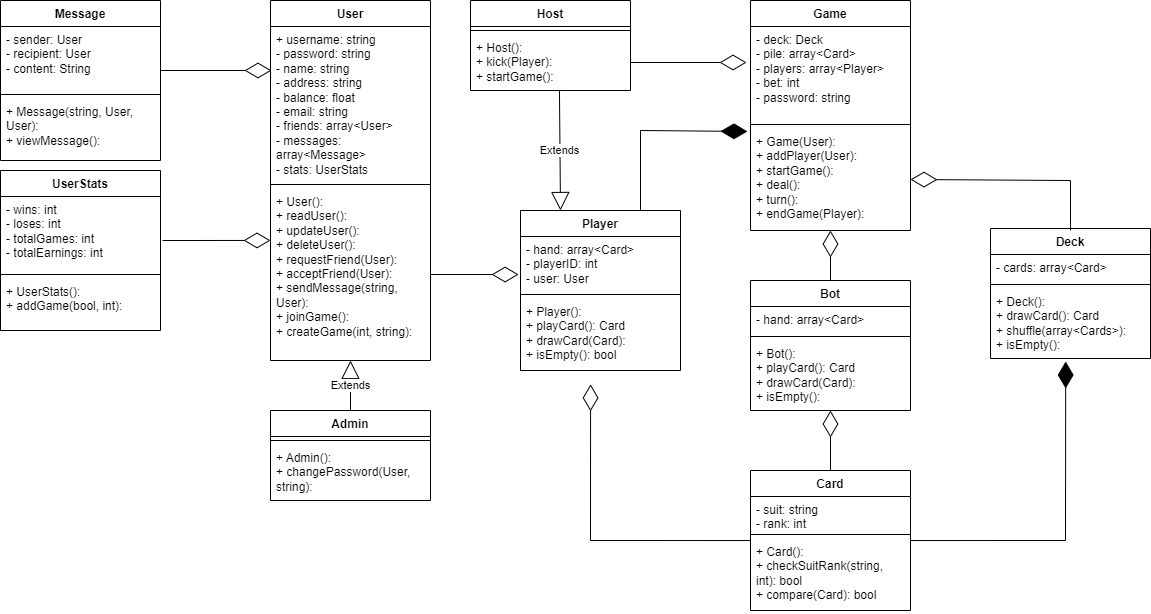
\includegraphics[width=\textwidth]{Crazy8sUML.png}
    \caption{UML Diagram of the Final System Architecture}
    \label{fig:uml_diagram}
\end{figure}
\section{Testing}

%[[ include test plan and coverage data 

%Briefly describe how you incorporated testing into each two week coding iteration. 
%What tool(s) proved useful? 
%What went well in terms of testing?
%What did not?]]

\subsection{Testing with Jest}

For sprint 1, our main focus was getting the website up and running, so all else, including testing, was a bit of an afterthought. Plus, the website was not very complicated at that point, so we were able to see if things were not working pretty quickly. Will set up Jest and wrote a few tests for the account pages and database functionality. However, the tests for the frontend encountered a lot of issues with mocking the various dependencies like socketio, and some components could not be tested as a result. 

In sprint 2, Jack wrote comprehensive tests for the backend game functionality, reaching almost 100\% test coverage on those classes. However, we did not have enough time to expand on the frontend tests.

For sprint 3, we focused a lot more on testing, though it took a significant amount of time and we encountered a lot of issues with it. Victoria combined the tests on the backend and frontend so that Jest could generate a comprehensive coverage report. Additionally, she wrote tests for the CreateGame page, Home page, Join Game page, and Game page, reaching 70-80\% coverage for those pages. A helpful tool for this was AI, as it could write tests much faster than a person could, and tests were extremely time consuming to write. However, we encountered numerous issues with Jest not detecting website components which decreased progress greatly. Additionally, AI tests needed to be looked over and debugged to ensure that they worked properly, which took more time. In the end, we were not able to get a proper amount of coverage for a signifigant quantity of the webpages and their components due to time limitations. Our code-generated coverage report is shown in figure \ref{fig:sprint3tests}. Each team member's approximate coverage is shown in table \ref{fig:coverage}. We were unable to determine the exact coverage for each member as it would take a while to accurately determine what percentage of each file was written by who and how much of it was covered by each test. Branch coverage was around 40 percent.

\subsection{Internal Code Quality}

Since each person worked on a different area of the website corresponding to the UI, server, and database, it was important that the code was consistent and well-documented. We accomplished this by writing comments specifying the parameters and purpose of each function, as well as using the camel case naming convention for variables and functions. Any unnecessary or redundant code was cleaned up to ensure that the files are as short as possible. However, there are some inconsistencies in indentation and the HTML code embedded in react is not completely commented.

Additionally, we made sure to separate each main object into its own file where possible. Each of the game objects were originally located within the server file, but are now contained within their own class and file. Each frontend webpage and its functions are contained within their own files as well. The server file is still quite large, but it would be difficult to separate it into its own components due to the nature of the database and socketio dependencies.


\begin{table}[h]

\centering
\begin{tabular}{|c|c|c|}
\hline
\textbf{} & \textbf{Area}     & \textbf{Coverage} \\ \hline
Jack      & Game Functions    & $\sim$80\%        \\ \hline
Victoria  & Main UI           & $\sim$50\%        \\ \hline
Will      & Account Functions & $\sim$30\%        \\ \hline

\end{tabular}
\caption{\label{fig:coverage} Each team member's approximate code coverage.}
\end{table}

\begin{figure}[H]
\centering
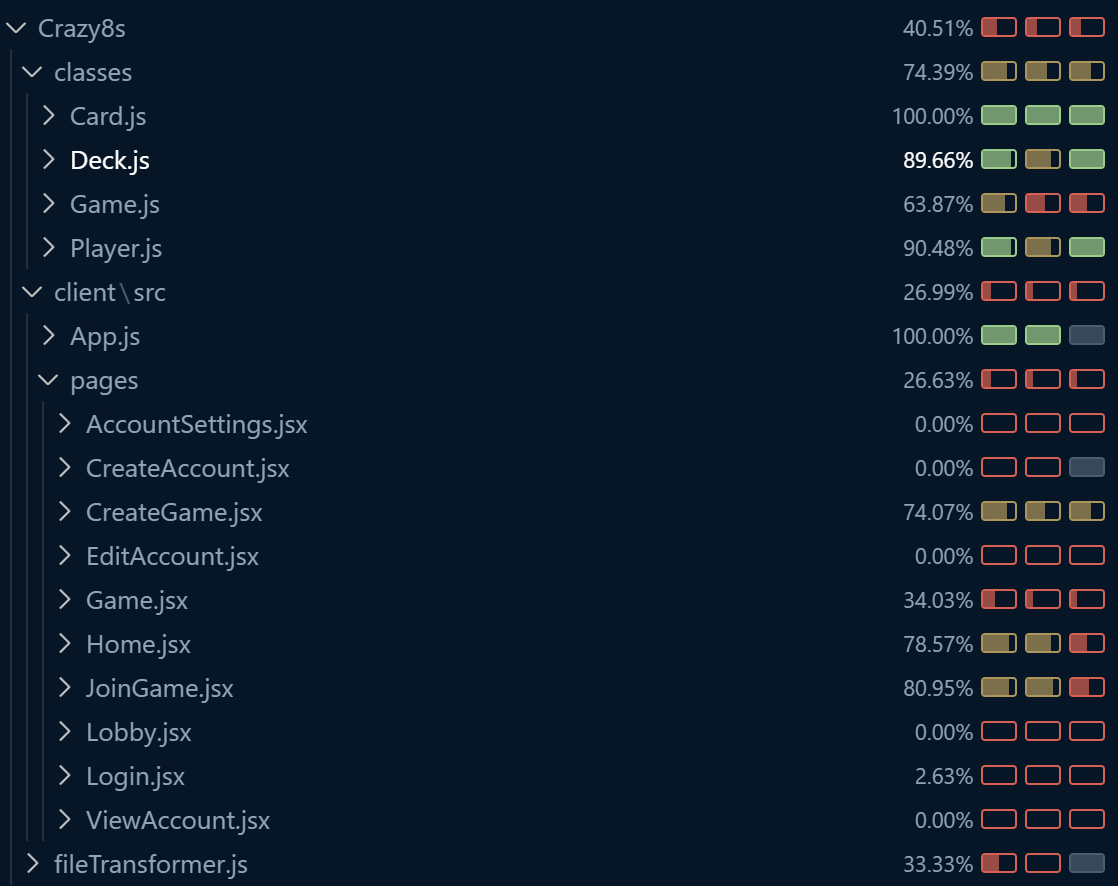
\includegraphics[width=\linewidth]{sprint3tests.png}
\caption{\label{fig:sprint3tests}The final test coverage.}
\end{figure}

 
\section{Persistence}

Explain how you store persistent (long-term) data. Not only what Database you are using
(which should be described earlier under Architecture and Design) but include the names of
your tables (SQL) or collections (NoSQL). The attributes of each table/collection. A visual
representation like an Entity Relationship Diagram (ERD) is much better than a plain textual
description. Remember that this information has probably changed since the beginning of
the semester. Thus, you should update your text and diagrams accordingly.

For our persistent data our group chose to use Firebase and a NOSQL database. Initially we chose SQL and were running our database locally on mySQL. This led to some issues as for multiplayer, we new we needed a fast and reliable database that could be hosted publicly online, not locally on one of our machines. We therefore made the switch to Firebase and likewise the switch to NOSQL. Our structure is comprised of four collections, Users, Messages, Conversations and Reports. Users contain their respective data as shown , keeping track of stats and balance. The conversation collection is made up of two user IDs combined to form a unique identifier for the conversation. Each conversation contains a collection of messages. A message contains the content, id of the sender, and a timestamp. Lastly there is a collection of reports, containing the issue and the name of the player being reported.\ref{fig:erd_diagram}

\begin{figure}[H]
    \centering
    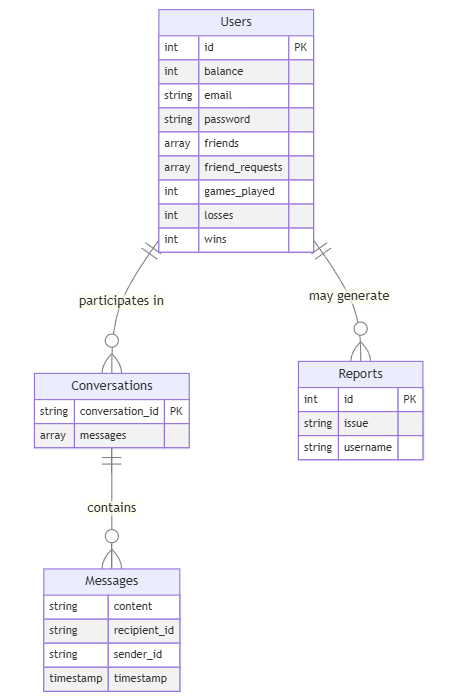
\includegraphics[scale=0.7]{finalERDdiagram.png}
    \caption{ERD Diagram of the Final Database Architecture}
    \label{fig:erd_diagram}
\end{figure}

\section{Reflections on the Project}

We learned a lot of lessons over the course of this project. One of the main things we learned was how to work and communicate effectively as a team. Our team did not have any specific leader, we did not need one because we each trusted each other to take on an equal amount of work and get things done when they needed to be done. We were well organized, and while we worked both separately and synchronously, it was never an issue as we communicated frequently. We did not have any notable disagreements that hindered progress.

The main strength of our group's execution of the project is that we each took on a specific software development role when building the website. Will worked on the database end, Jack worked on the server end, and Victoria worked on the front end. This allowed each of us to become an expert in our own topic, and assist other members if they needed to do something in a different area than their specialty. It also gave us a good way to divide up work between the group. 

The main barriers were our limited time and experience. Three two week sprints did not give us enough time, especially since we had to learn Javascript, React, and other topics relating to building and hosting a website. While three sprints may have been enough if we focused solely on the project, each of us had demanding classes and other priorities outside of class, forcing us to either sacrifice other classes or our completion of the project. While our website was perfectly functional in the end, it lacked the polish it could have had if we were able to work on it for a longer amount of time. If we had the knowledge we did today about the difficulties of the process, we could have done a few things differently. We could have prepared more for the project by learning the necessary topics beforehand, and spread work for each sprint throughout the week.

We learned a lot about working with the Agile process of software development. The sprints were a good layout for the project, but could have used either more time or a larger quantity of sprints. The Kanban board was very useful for keeping track of tasks and assigning them to each person. The user stories were difficult for the team to understand and work with, as we did not know how to format them as tasks to complete. Overall, the project was very informative, but a bit too much for the limited amount of time we had.



\subsection{AI Impact}
Each team member should write a paragraph or two on their experience using LLMs/AIs. If
you didn't make use of such tools, then write why you made that choice.

\subsubsection{Will}
My use of AI was mainly facilitated around being able to quickly learn new syntax given I was writing in a new language. Having never written in javascript, html or css before, I knew what I needed to do but the syntax was completely foreign to me which made it very hard to start. At the beginning I was able to use it to learn the syntax for classes, functions and other generic concepts that are consistent across programming languages. By doing this I was able to very quickly learn the syntax of all of the concepts that I would need for the project. Additionally, it was very helpful for transitioning my existing code from SQL to NOSQL when we made the switch to firebase. The AI was able to generate a basic structure for interacting with the database that I was able to modify as needed for each individual database function.

\subsubsection{Jack}
I used AI for a few things. Firstly, I used AI to learn React, JavaScript, HTML/CSS and SocketIO quickly. My experience with AI is that it gives incorrect or inefficient code, but it is great at giving the user a basic understanding of a topic. For example, when I wanted to learn JavaScript, I would ask how do var, const and let work. This would accelerate my learning, but it didn't give me much code. I also asked AI how to change the users page through code. That led me to finding the navigate function. The other way that I used AI was to debug my code. Sometimes, I would have an error, but I couldn't find it. So, I would ask AI to tell me where the bug is. This was inconsistent, but it saved me some time when it worked. 

\subsubsection{Victoria}

My use of AI was mainly to accelerate my learning of React, JavaScript, Jest, and CSS's syntax. Due to the time constraints of the project and my unfamiliarity with full stack development, I had to take shortcuts to learn how to complete my user stories on time. 

I used AI to give me a very quick and rough idea of what a certain section of code would look like, such as how a button executing a function would be implemented, what a class in CSS looked like to create a box in a certain area of the screen, how to display an image or video, how to write a test in Jest for a component in React, etc. This allowed me to comprehend the syntax much faster than checking documentation or tutorials and learning by trial and error. Once I had seen an example of how a section of code would look like, I was able to understand it, build on it, and use the topics in other sections of the project without the assistance of AI. 

I also used AI in the case of writing tests, as writing hundreds of tests by hand would have been far too time consuming. However, I spent a lot of time debugging the AI's attempts at writing tests, so it may have taken equal or less time to write the tests myself.

%\section{References}
%\bibliographystyle{plain}
%\bibliography{references}

%
\section{\LaTeX ``Tutorial''}

OMIT this section in production, but here is some sample \LaTeX~to munch on.

Use the table environment to include tables.
Be sure to keep the label and caption below the tabular!

Setting up tables can be annoying. You can also set it up in excel and then
copy it into \textsf{https://www.tablesgenerator.com} to generate the latex. 



\begin{table}[h!]
    \centering
    \begin{tabular}{|c|c|c|c|c|}
    \hline
      Risk   & Impact & Priority  & Overall Rating  & Mitigation \\
         &  &  &  & \\\hline
         &  &  &  & \\\hline
         &  &  &  & \\\hline
    \end{tabular}
    \caption{Risks to the software.}
    \label{tab:risks}
\end{table}

Table~\ref{tab:risks} overviews the risk relevant to our project.


Use the figure environment to include images such as \textsf{.png} in your latex document. \\

\begin{figure}[!bh]
\centering
\includegraphics[width=0.33\textwidth]{figures/sb.png} \\
\caption{Class Diagram for Sponge Bob's Best Christmas Ever.}
\label{fig:class}
\end{figure}

Figure~\ref{fig:class} shows the high-level class diagram.


\begin{figure}[!bht]
\begin{lstlisting}[language=Java]
public static void main(String [] args)
{
  System.out.println("Hello World!");
}
\end{lstlisting}
\caption{Hello Example.}
\label{fig:hello}
\end{figure}

Figure~\ref{fig:hello} shows the code used to print hello.
\textbf{Note that you writeup should include code sparingly.
The details of the code are not its focus.}



\end{document}

